\documentclass[12pt]{article}


\newcommand{\red}[1]{\textcolor{red}{#1}}
\newcommand{\blue}[1]{\textcolor{blue}{#1}}
\newcommand{\magenta}[1]{\textcolor{magenta}{#1}}
%------------------------packages-----------------------------
\usepackage{booktabs}
\usepackage[mathscr]{eucal}
\usepackage[cmex10]{amsmath}
\usepackage{epsfig,epsf,psfrag}
\usepackage{amssymb,amsthm,amsfonts,latexsym}
\usepackage{graphicx,xcolor,url,overpic}
\usepackage{array}%array and tabular environments
\usepackage{verbatim}
\usepackage{bm}
\usepackage{algorithm}
\usepackage{algpseudocode}
\usepackage{enumitem}
\setlist[itemize]{itemsep=0.25em, topsep=0.5em, parsep=0pt, partopsep=0pt, leftmargin=*}
\usepackage{textcomp}
\usepackage{mathrsfs}
\usepackage{hyperref}
\usepackage{epstopdf}
\usepackage{subfigure}
\usepackage{acronym}
\usepackage{diagbox}
\usepackage{listings}
\usepackage{tikz}
\usetikzlibrary{graphs, positioning, quotes, shapes.geometric}
\usepackage{thmtools, thm-restate}
%-----------------------------------------------------



\newcommand\independent{\protect\mathpalette{\protect\independenT}{\perp}}
\def\independenT#1#2{\mathrel{\rlap{$#1#2$}\mkern2mu{#1#2}}}
\newcommand{\openone}{\leavevmode\hbox{\small1\normalsize\kern-.33em1}}

%% To produce a tilde in url
\catcode`~=11 \def\UrlSpecials{\do\~{\kern -.15em\lower .7ex\hbox{~}\kern .04em}} \catcode`~=13

\allowdisplaybreaks[4]

\newcommand{\snr}{\mathsf{snr}}
\newcommand{\inr}{\mathsf{inr}}

\newcommand{\nn}{\nonumber}
\newcommand{\cequal}{\stackrel{\mathrm{c}}{=}}
\newcommand{\dequal}{\stackrel{\mathrm{d}}{=}}

\def\tv{\mathop{\mathrm{TV}}}
\newcommand{\unif}{{\text{Unif}}}
\newcommand{\kl}{D_{\mathrm{kl}}}
\newcommand{\md}{{\text{md}}}
\newcommand{\rd}{{\mathrm{d}}}
\newcommand{\rE}{{\text{{\tiny E}}}}
\newcommand{\rc}{{\mathrm{c}}}
\newcommand{\TD}{{\mathrm{TD} } }
\newcommand{\init}{{\text{init}}}
\newcommand{\proj}{\text{Proj}}
\newcommand{\err}{{\epsilon}}
\newcommand{\phic}{\iota}
%\newcommand{\gap}{\text{Gap}}
\newcommand{\DD}{\mathbb{D}}

% Calligraphic stuff
\newcommand{\calA}{\mathcal{A}}
\newcommand{\calB}{\mathcal{B}}
\newcommand{\calC}{\mathcal{C}}
\newcommand{\calD}{\mathcal{D}}
\newcommand{\calE}{\mathcal{E}}
\newcommand{\calF}{\mathcal{F}}
\newcommand{\calG}{\mathcal{G}}
\newcommand{\calH}{\mathcal{H}}
\newcommand{\calI}{\mathcal{I}}
\newcommand{\calJ}{\mathcal{J}}
\newcommand{\calK}{\mathcal{K}}
\newcommand{\calL}{\mathcal{L}}
\newcommand{\calM}{\mathcal{M}}
\newcommand{\calN}{\mathcal{N}}
\newcommand{\calO}{\mathcal{O}}
\newcommand{\calP}{\mathcal{P}}
\newcommand{\calQ}{\mathcal{Q}}
\newcommand{\calR}{\mathcal{R}}
\newcommand{\calS}{\mathcal{S}}
\newcommand{\calT}{\mathcal{T}}
\newcommand{\calU}{\mathcal{U}}
\newcommand{\calV}{\mathcal{V}}
\newcommand{\calW}{\mathcal{W}}
\newcommand{\calX}{\mathcal{X}}
\newcommand{\calY}{\mathcal{Y}}
\newcommand{\calZ}{\mathcal{Z}}

\newcommand{\hatcalA}{\hat{\calA}}
\newcommand{\hatcalB}{\hat{\calB}}
\newcommand{\hatcalC}{\hat{\calC}}
\newcommand{\hatcalD}{\hat{\calD}}
\newcommand{\hatcalE}{\hat{\calE}}
\newcommand{\hatcalF}{\hat{\calF}}
\newcommand{\hatcalG}{\hat{\calG}}
\newcommand{\hatcalH}{\hat{\calH}}
\newcommand{\hatcalI}{\hat{\calI}}
\newcommand{\hatcalJ}{\hat{\calJ}}
\newcommand{\hatcalK}{\hat{\calK}}
\newcommand{\hatcalL}{\hat{\calL}}
\newcommand{\hatcalM}{\hat{\calM}}
\newcommand{\hatcalN}{\hat{\calN}}
\newcommand{\hatcalO}{\hat{\calO}}
\newcommand{\hatcalP}{\hat{\calP}}
\newcommand{\hatcalQ}{\hat{\calQ}}
\newcommand{\hatcalR}{\hat{\calR}}
\newcommand{\hatcalS}{\hat{\calS}}
\newcommand{\hatcalT}{\hat{\calT}}
\newcommand{\hatcalU}{\hat{\calU}}
% \usepackage{refcheck}
\usepackage{mathtools}
% \mathtoolsset{showonlyrefs}
\usepackage{bbm}
\usepackage{svg}
\usepackage[round]{natbib}
\usepackage{geometry}
\geometry{a4paper,scale=0.8}
\usepackage{acronym}
\acrodef{mab}[MAB]{Multi-Armed Bandit}

\theoremstyle{plain}
\newtheorem{theorem}{Theorem}[section]
\newtheorem{proposition}[theorem]{Proposition}
\newtheorem{lemma}[theorem]{Lemma}
\newtheorem{corollary}[theorem]{Corollary}
\theoremstyle{definition}
\newtheorem{definition}[theorem]{Definition}
\newtheorem{assumption}[theorem]{Assumption}
\theoremstyle{remark}
\newtheorem{remark}[theorem]{Remark}
\newtheorem{requirement}{Requirement}


\title{UCUG1903 26 Spring Project Report}
\author{Jiongxu CHEN, Xiangqian WANG, Yiqiu LIU}
\date{May 2026}

\begin{document}

\maketitle

\section{Introduction}
\label{sec:intro}

1980s game and home-computer audio was shaped by scarce ROM, weak integer CPUs, and simple converters, not by general-purpose sampling pipelines.
Engineers relied on \emph{command-driven} sound chips: the CPU sends coarse parameters (frequency, level, waveform type) and the chip synthesizes audio in real time (Figure~\ref{fig:command-driven}).

This report summarizes that design space and its perceptual counterpart.
Section~\ref{sec:waveforms} reviews square, sawtooth, and LFSR-style noise---and why sine generation was rarely affordable---then Section~\ref{sec:perception} relates those signals to timbre, pitch (equal temperament), and loudness (decibels).
Section~\ref{sec:web} describes a browser demo (Web Audio, piano-roll editing, WAV export) that echoes the same primitives without original hardware.


\section{Hardware Constraints in the 1980s}
In the 1980s, game consoles and home computers faced severe hardware limitations. Storage media, such as ROM cartridges or tapes were measured in kilobytes, not megabytes. Processing power was also extremely low: CPUs were only 4‑bit or 8‑bit and lacked hardware multipliers. So they could not perform complex floating‑point calculations.

\begin{figure}[h]
\centering
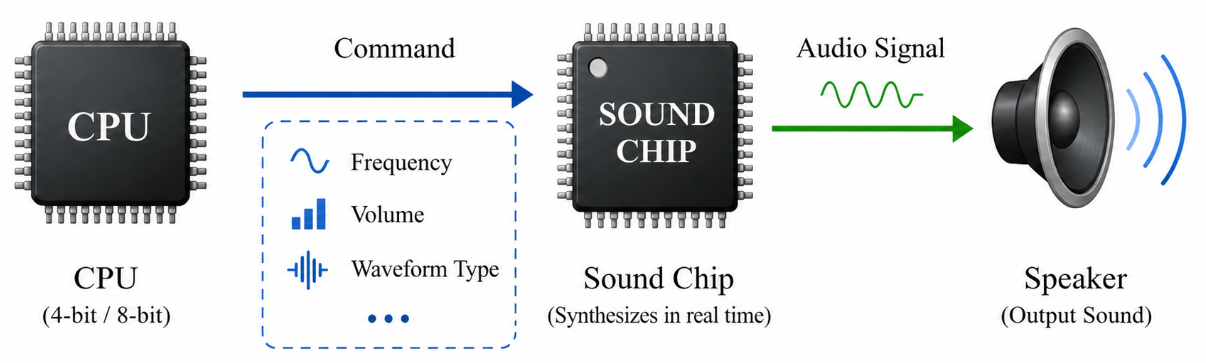
\includegraphics[width=0.65\linewidth]{pictures/command-driven.png}
\caption{Block diagram of command‑driven audio: CPU $\to$ Commands $\to$ Sound Chip $\to$ Speaker.}
\label{fig:command-driven}
\end{figure}

To work within these constraints, engineers invented command‑driven audio (Figure ~\ref{fig:command-driven}). Instead of streaming heavy audio data, the CPU sent simple commands (frequency, volume, waveform type) to a dedicated sound chip, which synthesized the sound in real time. This saved precious storage and CPU cycles.


\section{Three Basic Waveforms and Why No Sine Wave?}
\label{sec:waveforms}

Sound chips in the 1980s generated three fundamental waveforms (Figure~\ref{fig:three-waves}) using simple digital circuits.

\begin{itemize}
  \item \textbf{Square wave.} Generated by a frequency divider.
  The chip counts system clock cycles and toggles between high and low voltage at a desired frequency.
  \item \textbf{Sawtooth wave.} Created with a digital accumulator.
  The accumulator repeatedly adds a fixed step.
  When it reaches the maximum, it resets instantly to zero.
  \item \textbf{Noise wave.} Produced by a linear feedback shift register (LFSR), a pseudo-random circuit that uses XOR feedback to generate a random stream of bits.
\end{itemize}

These three waveforms, requiring only a few logic gates and counters, became the building blocks of nearly all 8-bit game audio in the 1980s.

Although the sine wave is the most fundamental waveform in signal processing, it was absent from these chips.
Generating a sine wave was simply too expensive for 1980s hardware.

\begin{itemize}
  \item \textbf{Computational cost.} A sine wave requires trigonometric functions or Taylor-series expansion.
  A slow 4-bit or 8-bit CPU with no hardware multiplier could not perform such calculations in real time.
  \item \textbf{Hardware limitation.} A smooth sine wave needs a high-precision DAC.
  Most sound chips at that time had only primitive counter-based DACs, or no DAC at all---they produced step-like outputs rather than smooth curves.
  \item \textbf{Memory waste.} An alternative is to pre-compute sine values and store them in a lookup table (LUT), which would consume valuable ROM measured in kilobytes.
\end{itemize}

\begin{figure}[htbp]
  \centering
  \subfigure[Square wave.\label{fig:square}]{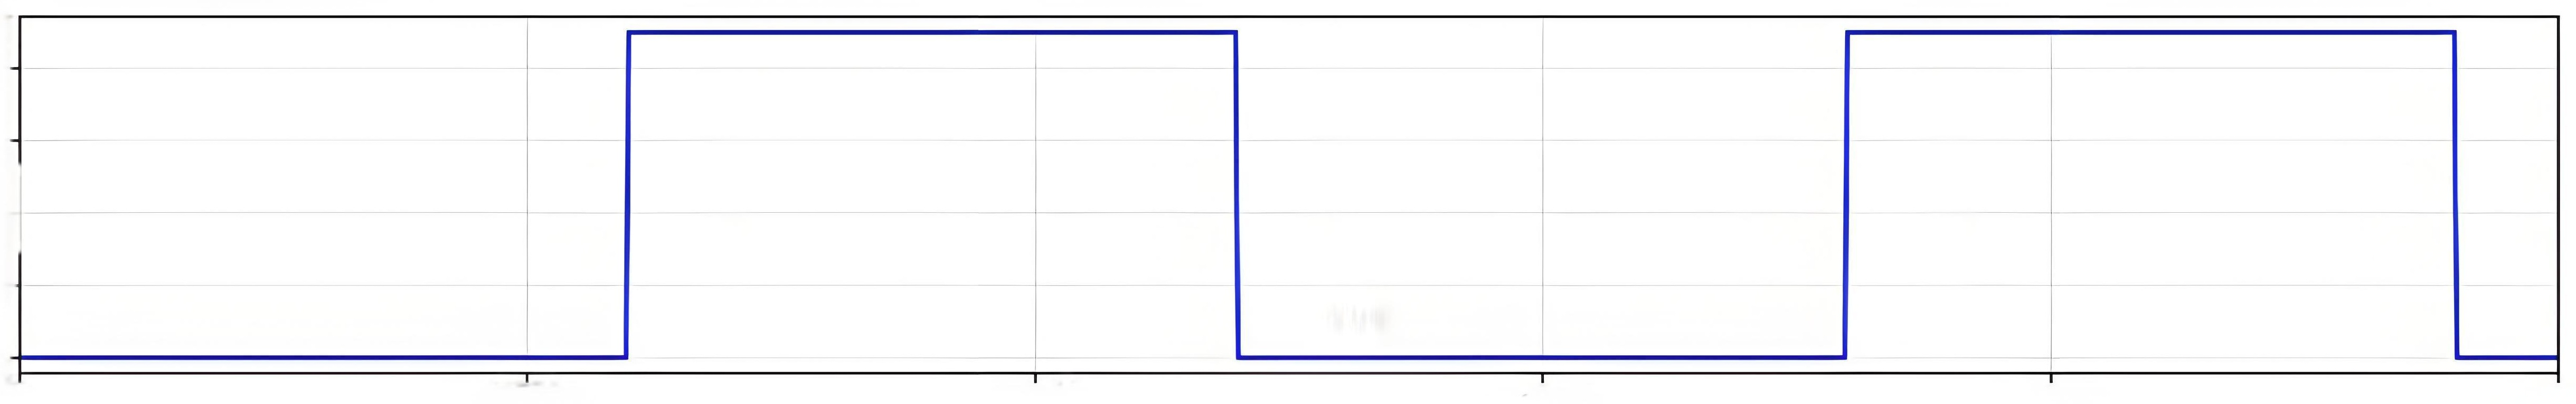
\includegraphics[width=0.32\linewidth]{pictures/square.png}}
  \hfill
  \subfigure[Sawtooth wave.\label{fig:sawtooth}]{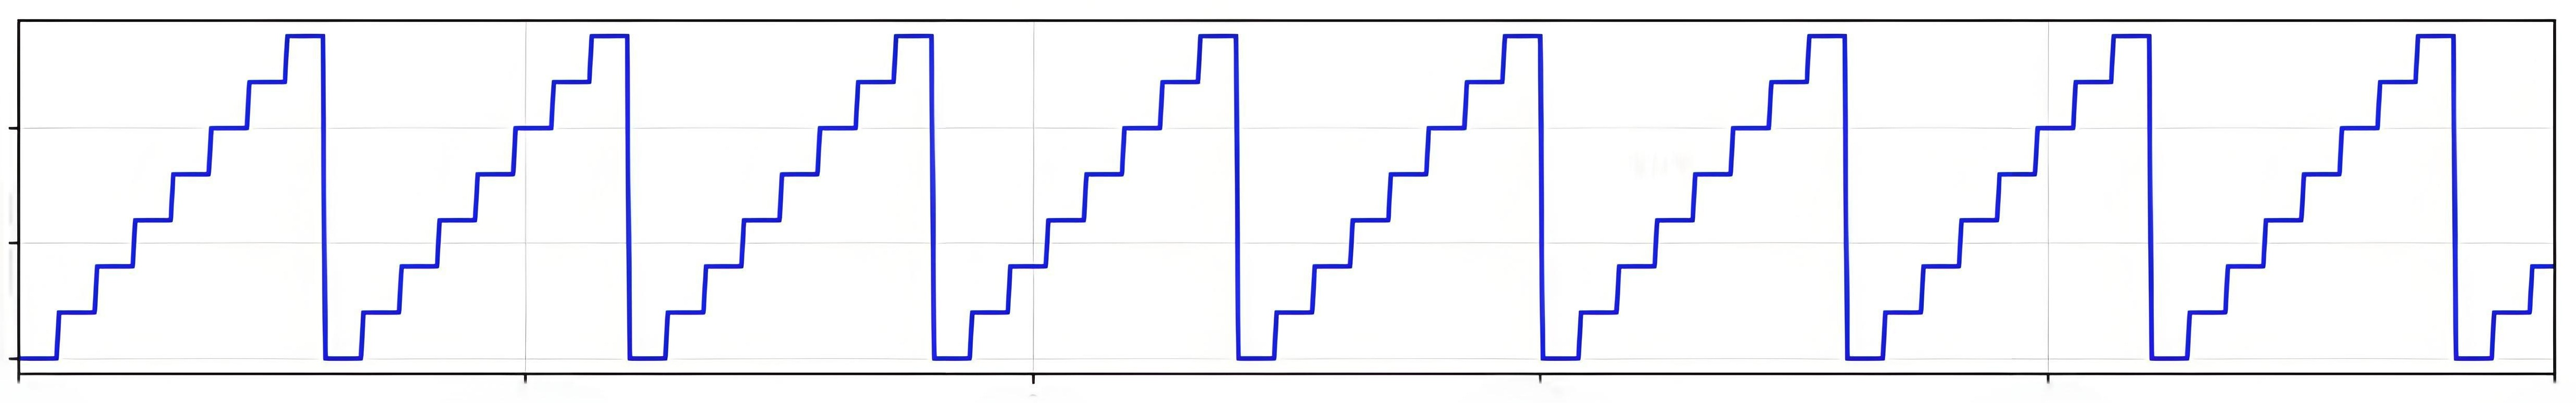
\includegraphics[width=0.32\linewidth]{pictures/sawtooth.png}}
  \hfill
  \subfigure[Noise wave.\label{fig:noise-wave}]{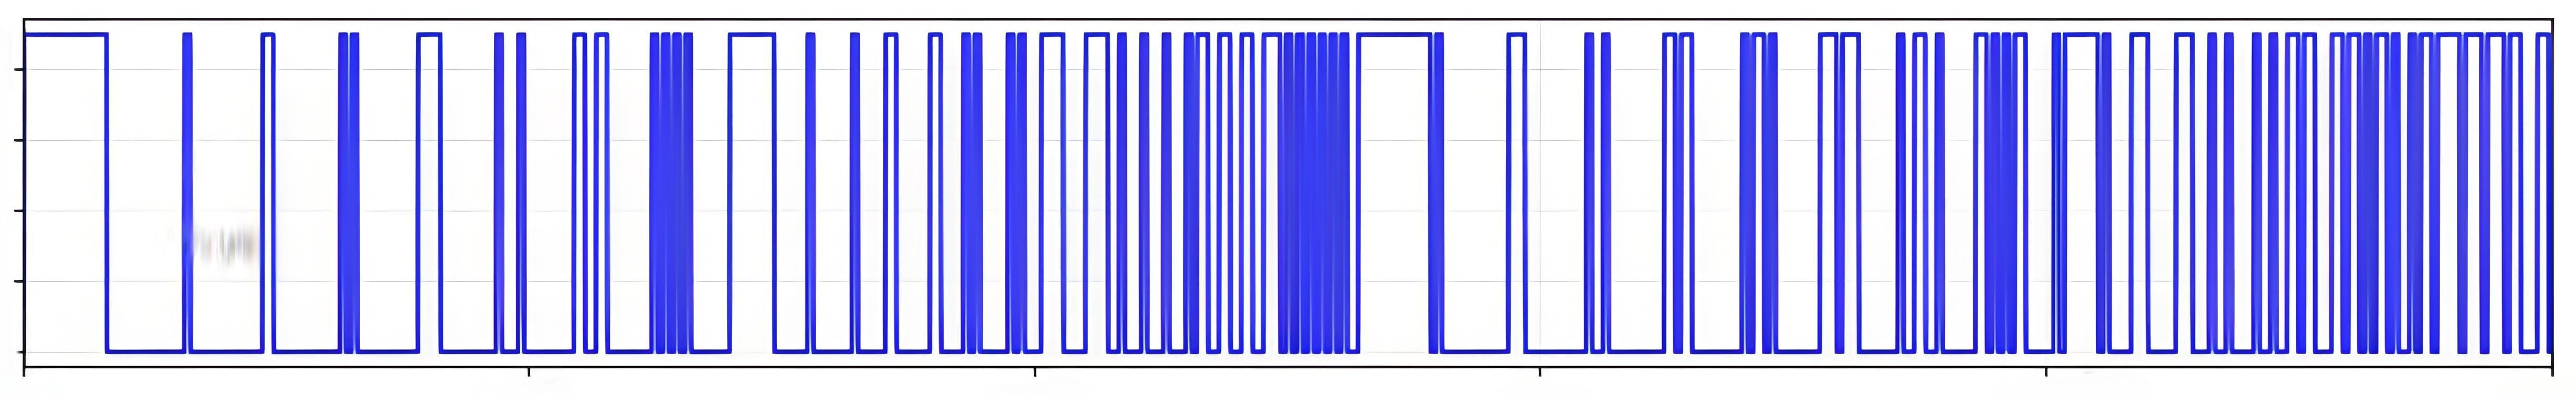
\includegraphics[width=0.32\linewidth]{pictures/noise.png}}
  \caption{Three basic waveforms.}
  \label{fig:three-waves}
\end{figure}


\section{From Basic Waveforms to Musical Perception}
\label{sec:perception}

The previous section described how early sound chips generated a limited set of waveforms under hardware constraints.
These signals become meaningful in music once listeners perceive them; the link between synthesis and musical expression can be summarized by three attributes---timbre, pitch, and loudness.

\subsection{Timbre: Waveform as Sound Color}

Timbre mainly depends on waveform shape.
Even when pitch and loudness match, different waveforms still sound different.
The three primitives on typical 1980s sound chips mapped to distinct musical roles:

\begin{itemize}
  \item \textbf{Square wave.} Produces a clear, distinct tone, suitable for lead melodies and simple harmonies.
  \item \textbf{Sawtooth wave.} Sounds fuller and more stable---often used for bass lines.
  \item \textbf{Noise wave.} Lacks stable pitch---used for percussion and drum-like effects.
\end{itemize}

Figure~\ref{fig:three-waves} illustrates these waveform shapes and their timbral basis.

\subsection{Pitch: Frequency Determines Musical Notes}

Pitch is determined by frequency: a higher carrier frequency is heard as a higher note.
In twelve-tone equal temperament, one semitone corresponds to the frequency ratio $2^{1/12}$, so an interval of $n$ semitones scales frequency by $(2^{1/12})^n$.
Table~\ref{tab:c-major-scale} lists selected C-major scale frequencies as an example.

\begin{table}[htbp]
  \centering
  \caption{Frequencies of selected notes in the C major scale.}
  \label{tab:c-major-scale}
  \begin{tabular}{cccc}
    \toprule
    \textbf{Syllable} & \textbf{Frequency (Hz)} & \textbf{Interval vs.\ prev.} & \textbf{Frequency ratio} \\
    \midrule
    do & 261.63 & --- & --- \\
    re & 293.66 & 2 semitones & $(2^{1/12})^2$ \\
    mi & 329.63 & 2 semitones & $(2^{1/12})^2$ \\
    fa & 349.23 & 1 semitone & $2^{1/12}$ \\
    sol & 392.00 & 2 semitones & $(2^{1/12})^2$ \\
    \bottomrule
  \end{tabular}
\end{table}

As Table~\ref{tab:c-major-scale} shows, note spacing is multiplicative rather than additive in frequency.

\subsection{Loudness: Amplitude Controls Perceived Volume}

Loudness is dominated by amplitude: larger waveform excursions are heard as louder sounds.
Figure~\ref{fig:three-amplitudes} shows three sawtooth waves sharing the same frequency but different peak amplitudes; Table~\ref{tab:loudness-comparison} lists the corresponding amplitude ratios.

The level difference between amplitudes $A_1$ and $A_2$ may be expressed in decibels (dB) as
\[
L = 20 \log_{10}\!\left(\frac{A_2}{A_1}\right).
\]
For amplitude ratios $1{:}2{:}4$, each doubling yields about $6.02~\mathrm{dB}$, as plotted in Figure~\ref{fig:three-amplitudes} and summarized in Table~\ref{tab:loudness-comparison}.
Thus loudness aligns more naturally with a logarithmic amplitude scale than a linear one.

\begin{figure}[htbp]
  \centering
  \subfigure[Amplitude $=0.20$.\label{fig:loudness-1x}]{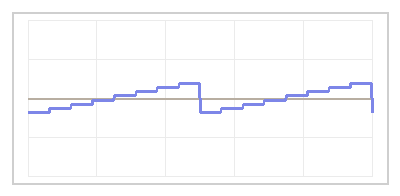
\includegraphics[width=0.32\linewidth]{pictures/loudness_comparison_1x.png}}
  \hfill
  \subfigure[Amplitude $=0.40$.\label{fig:loudness-2x}]{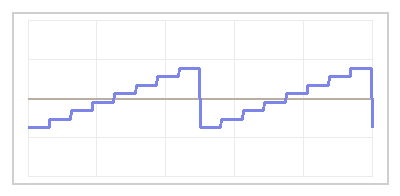
\includegraphics[width=0.32\linewidth]{pictures/loudness_comparison_2x.png}}
  \hfill
  \subfigure[Amplitude $=0.80$.\label{fig:loudness-4x}]{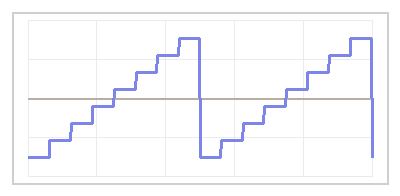
\includegraphics[width=0.32\linewidth]{pictures/loudness_comparison_4x.png}}
  \caption{Sawtooth waveforms at the same frequency with different peak amplitudes.}
  \label{fig:three-amplitudes}
\end{figure}

\begin{table}[htbp]
  \centering
  \caption{Relative amplitude and decibel levels for sawtooth waves with peaks $0.20$, $0.40$, and $0.80$.}
  \label{tab:loudness-comparison}
  \begin{tabular}{cccc}
    \toprule
    Amplitude & Ratio to $0.20$ & Level vs.\ $0.20$ & Increment (dB) \\
    \midrule
    $0.20$ & $1{:}1$ & $0.00$ & --- \\
    $0.40$ & $2{:}1$ & $6.02$ & $6.02$ \\
    $0.80$ & $4{:}1$ & $12.04$ & $6.02$ \\
    \bottomrule
  \end{tabular}
\end{table}


\section{Building the Web-Based Interactive Demo}
\label{sec:web}

We built a \emph{static} site in \texttt{web/} so lecture ideas---\emph{pitch vs.\ frequency}, \emph{waveform vs.\ timbre}, and \emph{simple noise}---can be tried in the browser with no backend.
The client uses HTML5, CSS, JavaScript, and the \textbf{Web Audio API}; real-time audition and offline export share one synthesis path.
Staying static avoided servers, credentials, and databases yet still scales for classroom traffic once GitHub Pages hosts the assets.
File boundaries (\texttt{app.js} vs.\ \texttt{audio-engine.js}) mirrored how we split UI work from DSP during the project.

\subsection{Features and Stack}

Users edit $1$--$16$ steps: duration on a $0.2$--$1.0\,\mathrm{s}$ grid (step $0.1$), pitch on thirteen C-major solf\`{e}ge degrees from low \textit{sol} to high \textit{mi} with Hz labels, waveform (square or sawtooth), and optional noise.
A piano-roll score plots time left to right; colors distinguish waveforms, hatched blocks mark noise, and clicking a block jumps to that step.
During playback an output waveform shows the mix; a master gain slider and \textbf{Export WAV} complete the listen--inspect--save loop.
The score and oscilloscope connect what listeners hear with a time-aligned trace for screenshots or archives.
A preset loader and \texttt{web/qr-site.png} simplify demos and mobile access; GitHub Actions publishes \texttt{web/} from repository \url{https://github.com/Displace1/UCUG1903} (see \texttt{.github/workflows/deploy-pages.yml} and \texttt{README.md}).
Roles of source files are listed in Table~\ref{tab:web-files}.

\begin{table}[htbp]
  \centering
  \caption{Web source files and responsibilities.}
  \label{tab:web-files}
  \begin{tabular}{@{}ll@{}}
    \toprule
    Path & Role \\
    \midrule
    \texttt{web/index.html} & Structure, controls, canvases \\
    \texttt{web/style.css} & Layout, theme, readability \\
    \texttt{web/app.js} & UI state, score/wave drawing, input, engine calls \\
    \texttt{web/audio-engine.js} & Waves, noise, play/stop, WAV render \\
    \texttt{web/song-schema.js} & Timeline and frequency helpers \\
    \texttt{web/default-song.json} & Default / demo sequence \\
    \bottomrule
  \end{tabular}
\end{table}

\subsection{Architecture and Core Logic}

Presentation lives in \texttt{app.js} (DOM, canvases, and state).
The module \texttt{audio-engine.js} writes samples, and \texttt{song-schema.js} negotiates timing and frequency fields between them.
Figure~\ref{fig:web-arch} sketches the data flow.
Square and sawtooth are synthesized per audio-rate sample; noise follows a console-style \textbf{15-bit LFSR} with low-pass shaping.
Tonal and noise buses are scaled (e.g.\ $1/\sqrt{2}$) before summing to limit clipping, following \texttt{README.md}.
Canvas hit-testing maps clicks back to controls.
Offline \texttt{AudioContext} rendering wraps the same buffers as live playback into standard WAV, so exported audio matches the synthesized timeline aside from buffering delay.

\begin{figure}[htbp]
  \centering
  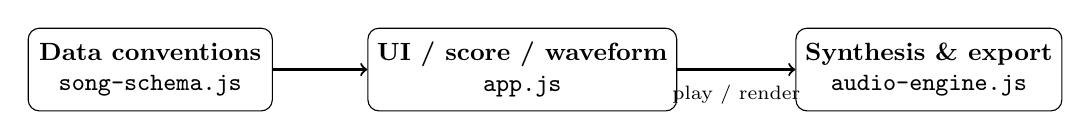
\begin{tikzpicture}[
    box/.style={draw, rounded corners, align=center, minimum width=3.1cm, minimum height=1.05cm},
    font=\small
  ]
    \node[box] (schema) {\textbf{Data conventions}\\\texttt{song-schema.js}};
    \node[box, right=1.2cm of schema] (app) {\textbf{UI / score / waveform}\\\texttt{app.js}};
    \node[box, right=1.5cm of app] (audio) {\textbf{Synthesis \& export}\\\texttt{audio-engine.js}};
    \draw[->, thick] (schema) -- (app);
    \draw[->, thick] (app) -- node[midway, below=0.15cm, font=\scriptsize, inner sep=1pt] {play / render} (audio);
  \end{tikzpicture}
  \caption{Front-end modules and data flow.}
  \label{fig:web-arch}
\end{figure}

\subsection{Deployment}

Source and documentation reside at \url{https://github.com/Displace1/UCUG1903}.
Each push triggers GitHub Actions to deploy \texttt{web/} to GitHub Pages; the public demo is \url{https://displace1.github.io/UCUG1903/}.
Use \texttt{HTTPS} or a local HTTP server rather than \texttt{file://} for reliable audio.
The bundled QR code targets the same URL for classroom phones.


\section{Conclusion}
\label{sec:conclusion}

Retrospective game audio makes a compact case study in constrained signal processing.
Severely limited memory and arithmetic forced a decomposition of the problem---the CPU programs \emph{parameters}, while periodic dividers, accumulators, and feedback shift registers synthesize recognizable tones and noise bursts on dedicated hardware.
Against that backdrop, sine synthesis was disproportionately costly, so composers worked with edgy spectra that were cheap to emit yet still expressive inside short loops.

Connecting chip waveforms to \emph{timbre}, \emph{pitch}, and \emph{loudness} clarifies why a small toolkit could cover harmonic content, tempered scales via multiplicative frequency steps, and level changes well captured on a logarithmic (decibel) axis.
These links also explain hallmark musical roles: square tones for melodic lines, rich saw shapes for supportive bass registers, and aperiodic noise for percussive color.

Our static web synthesizer echoes the same pedagogical storyline.
By separating timeline data, UI canvases, and the audio engine, the demo aligns software structure with lecture emphasis on oscillator models, quantization of timing and pitch choices, scaled noise mixtures, and traceable WAV export for offline inspection.

Looking forward, the stack could incorporate additional wave-shaping motifs (duty-cycle variation, rudimentary envelopes) or juxtapose synthesized output with archival recordings---extensions that reuse the project's interactive loop of \emph{hear}, \emph{see}, and \emph{save}.


\end{document}

